%% Slides for ".NET Programming" by Chunyu Wang <chunyu@hit.edu.cn> %%

\part{ADO.NET 简介}
\begin{frame}
\frametitle{Outline}
\tableofcontents
\end{frame}

\section{ADO.NET 基础}

\begin{frame}
\frametitle{ADO.NET 基础}
\begin{block}{\textit{ActiveX Data Object .NET}}
  \CJKindent 由公共语言运行时 (\textit{CLR}) 管理的数据管理库,利用 XML 在应
  用程序之间进行数据交换。
\end{block}
\begin{itemize}
\item 便于创建高效、可靠基于 Internet 数据库应用程序
\item 应用程序根据需要连接数据库,如读取或更新时
\item 利于分布式数据访问,节省资源
\item 托管环境中运行,由 CLR 负责资源管理
\item 利用 XML 多种方式传递数据,便于数据交换
\item Visual Stuido 提供可视化数据组件
\end{itemize}
\end{frame}

\begin{frame}
\frametitle{Microsoft 数据访问技术回顾}
\begin{itemize}
\setlength{\itemsep}{8pt plus 1pt}
\item Open Database Connectivity (ODBC)
 % 第一个规范的数据访问技术
 % 只能访问关系数据,无法兼容非关系数据
\item Data Access Object (DAO)
 % 一组访问数据库的 COM 接口,直接访问数据库
 % 便于访问 Access, FoxPro, SQL Server
\item MFC ODBC and DAO classes
 % C++ 类库,但不够灵活,效率也不理想,因为层次太多
\item Remote Data Objects (RDO)
 % 层次多,效率低,因为仍使用 ODBC,使用受到限制
\item Object Linking and Embedding Database (OLE DB)
 % 支持多种数据源,使用灵活
 % 必须安装 OLE DB Provider,使用较复杂
\item ActiveX Data Objects (ADO)
 % 使用 COM 包装,使用较简单
 % 效率较高,使用较灵活
\end{itemize}
% \bigskip
% \pause 数据库的访问、管理等,是企业应用程序开发中的核心问题。
\end{frame}

\begin{frame}
\frametitle{ADO.NET 命名空间}

\begin{itemize}
\item ADO.NET 是 FCL 的一部分
\item 包含在程序集 System.Data.dll 中
\end{itemize}

\begin{tabular}{l|l}
\hline
\textbf{Namespaces} & \textbf{Description} \\
\hline
\small System.Data & 实现 ADO.NET 的类、接口、委托类型等 \\
\small System.Data.Common & 不同数据提供程序共享的类 \\
\small System.Data.Odbc & ODBC 数据提供程序 \\
\small System.Data.OleDb & OLE DB 数据提供程序 \\
\small System.Data.OracleClient & Oracle 数据提供程序 \\
\small System.Data.SqlClient & SQL Server 数据提供程序 \\
\small System.Data.Sql & 用于支持 SQL Server 的功能类库 \\
\hline
\end{tabular}
\end{frame}

\begin{frame}
\frametitle{ADO.NET 的结构}

\begin{itemize}
\item 两个核心组件:\textit{Data Provider} 和 \textit{Dataset}
\end{itemize}

\begin{center}
%  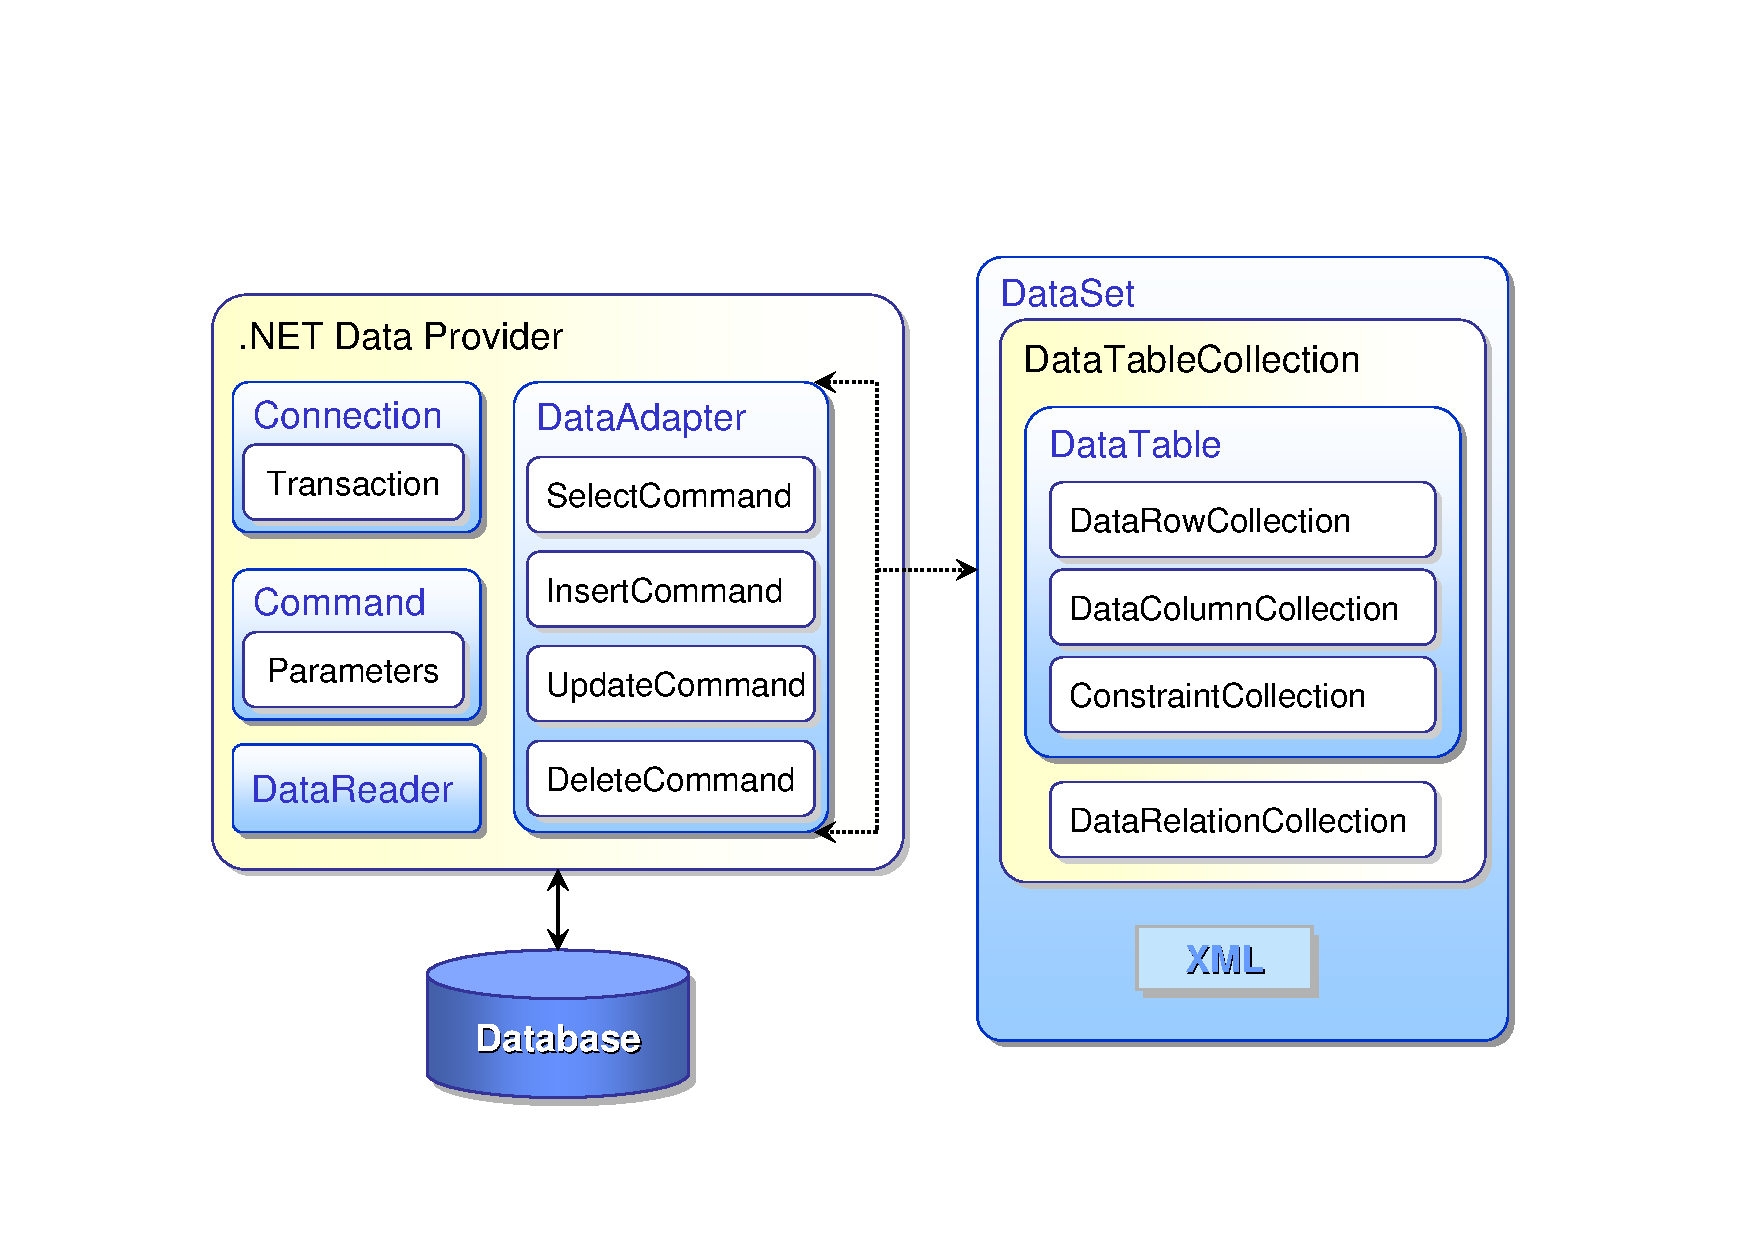
\includegraphics[scale=.46]{ado-arch}
  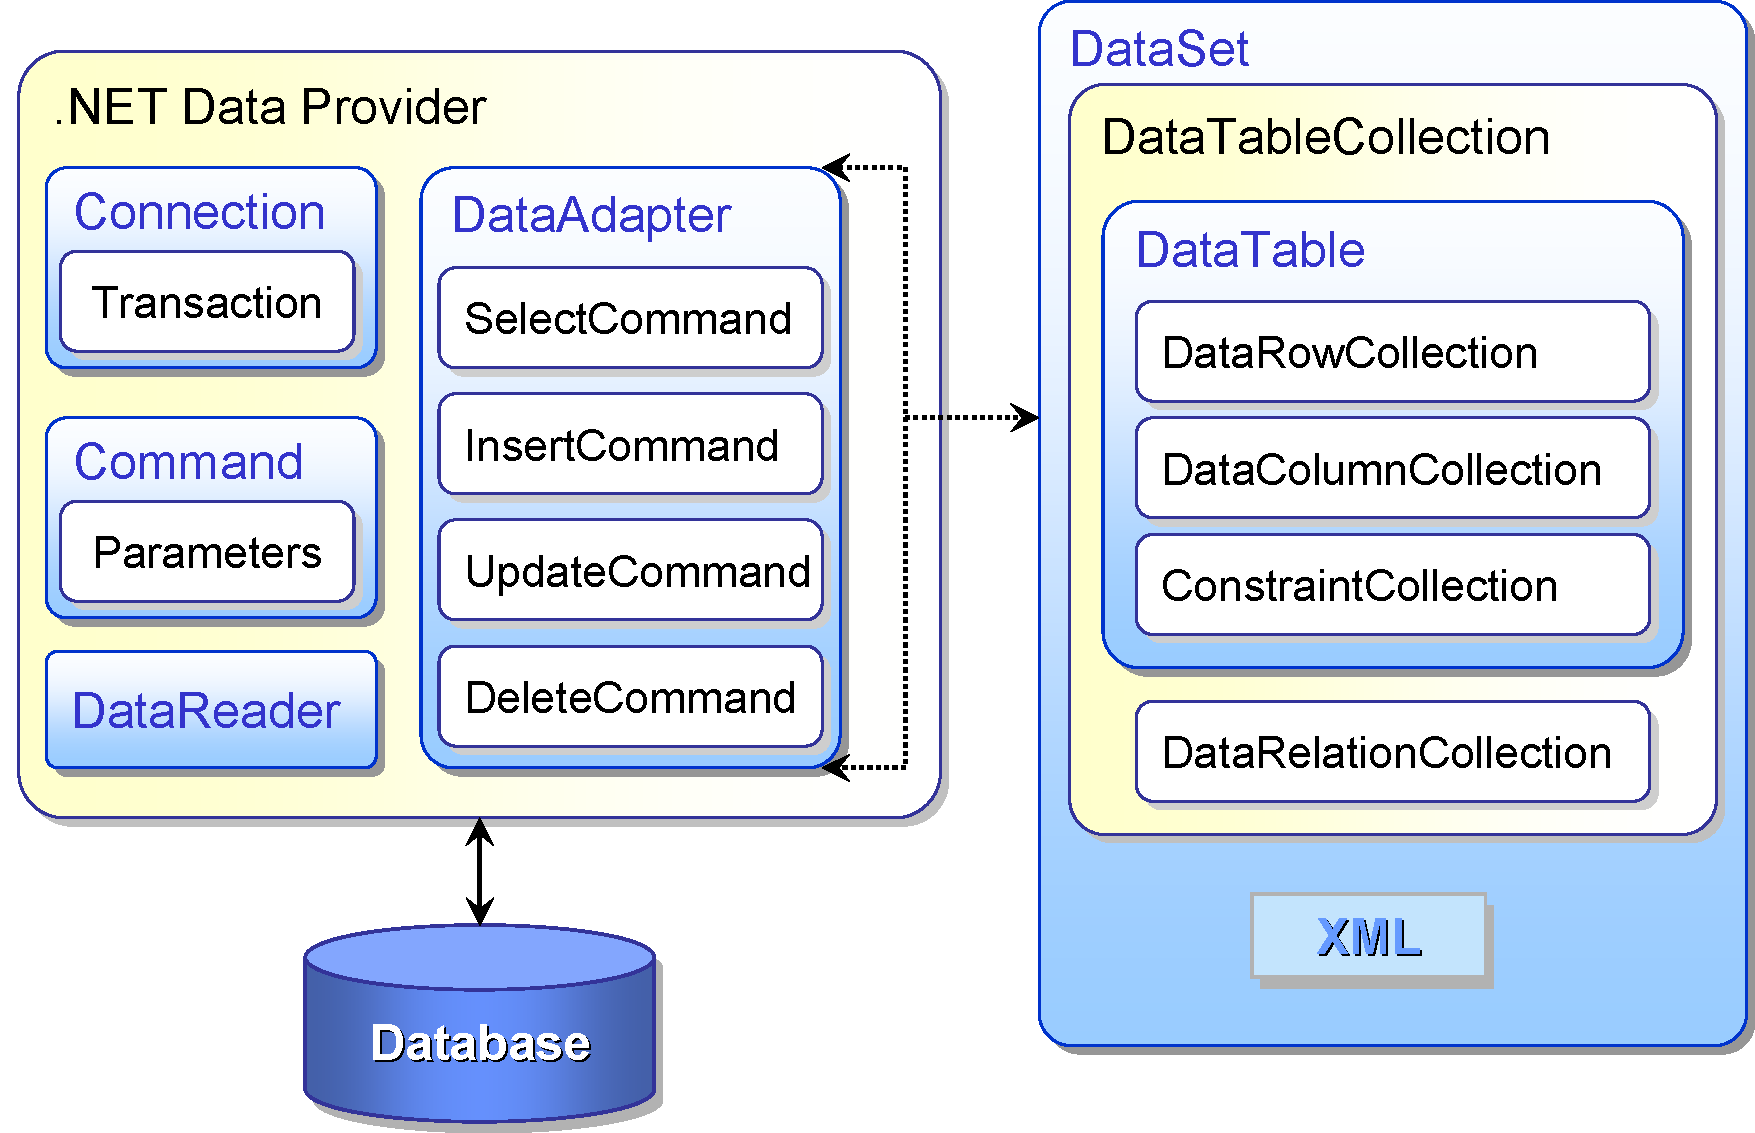
\includegraphics[scale=.46]{ado-arch-png}
\end{center}

\end{frame}

\section{Data Provider}

\begin{frame}
\frametitle{数据提供程序 (\textit{Data Provider})}
\begin{itemize}
\item 应用程序访问数据库依赖于 \textit{.NET Framework data provider}
\item 客户程序和数据提供程序,运行在 CLR 上
\item 数据提供程序可能依赖其它程序
\end{itemize}
\begin{center}
  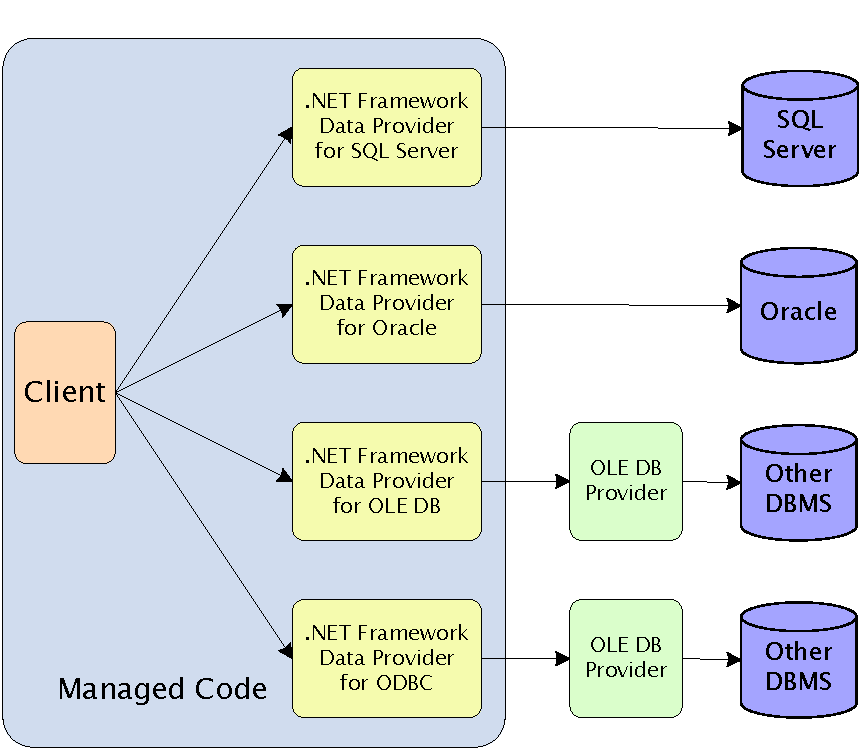
\includegraphics[scale=.5]{ado-provider}
\end{center}
\end{frame}

\begin{frame}
\frametitle{数据提供程序的功能}
\begin{itemize}
\item Connection 建立和释放连接,可用于启动事务
\item Command 执行 SQL 语句或存储过程
\item DataReader 只读、顺序的 (\textit{Sequential}) 直接访问库中数据
\item DataAdapter 创建并组装 DataSet 实例
\end{itemize}
\begin{center}
  %% Slides for ".NET Programming" by Chunyu Wang <chunyu@hit.edu.cn> %% -*- coding: utf-8 -*-

\begin{tikzpicture}[rounded corners, font=\sffamily\scriptsize, >=stealth]
\draw[fill=yellow!30, fill opacity=.5] (0,1.3) rectangle (6,6);
\draw[fill=blue!20, fill opacity=.8] (.2,1.5) rectangle (2.5,4.5);
\draw[fill=blue!20, fill opacity=.8] (2.7,1.5) rectangle (5.8,5.8);
\draw (1.35,4.1) node {\bf Client} (4.25,5.4) node {\bf .NET Framework}
(4.25,5.1) node {\bf Data Provoder};
\draw[fill=red!20] (3.75,4.5) ellipse (.8cm and .3cm) node {Connection};
\draw[fill=red!20] (4.8,3.85) ellipse (.8cm and .3cm) node {Command};
\foreach \x/\y in {1/3.5, 1.2/3.3, 1.4/3.1}
  \filldraw (\x,\y) node[draw=black,fill=white,minimum height=.5cm,minimum width=.8cm] {};
\draw (1.4,3.1) node[minimum height=.5cm,minimum width=.8cm] (row) {Rows};
\draw (4,3.1)  node[ellipse,draw,fill=red!20] (datar) {DataReader};
\draw (1.25,2.2) node[ellipse,draw,fill=orange!20] (datas) {DataSet};
\draw (4.5,2.2)  node[ellipse,draw,fill=red!20] (dataa) {DataAdapter};
\draw[fill=blue!20] (7.5,2.3) ellipse (.5cm and .15cm);
\fill[sharp corners,blue!20] (7,2.3) rectangle (8,3);
\draw[fill=blue!20] (7.5,3) ellipse (.5cm and .15cm);
\draw (7,2.3) -- (7,3) (8,2.3) -- (8,3);
\draw (7.5,2.6) node {DBMS};

\draw[->] (datar.200) ..  controls +(210:.5cm) and +(-30:.5cm) .. (row.-45);
\draw[->] (dataa.200) ..  controls +(210:.8cm) and +(-30:.5cm) .. (datas.-30);
\draw[->] (7,2.7) -- (datar.east);
\draw[->] (7,2.4) -- (dataa.east);
\end{tikzpicture}

\end{center}
\end{frame}

\begin{frame}
\frametitle{提供程序的命名空间}
% in System.Data.dll assembly
\begin{itemize}
\setlength{\itemsep}{8pt plus 1pt}
\item 特定的数据提供程序,位于不同的命名空间
\begin{itemize}
\setlength{\itemsep}{6pt plus 1pt}
\item System.Data.Odbc
\item System.Data.OleDb
\item System.Data.OracleClient
\item System.Data.SqlClient
\end{itemize}
\item 公共的数据提供程序
  \begin{itemize}
  \item System.Data.Common
  \smallskip
  \item 与其它提供程序共享的类和抽象基类
  \item 提供了通用编码的实现方式
  \end{itemize}
\end{itemize}
\end{frame}

\begin{frame}
\frametitle{SQL Server 的数据提供程序}

\begin{itemize}
\item System.Data.SqlClient 中
\item 在 .NET 上直接访问 SQL Server
\end{itemize}

  \begin{tabular}{l|l}
    \hline
    \textbf{Classes} & \textbf{Description} \\
    \hline
    \texttt{SqlConnection} & 建立与 SQL Server 的连接 \\
    \texttt{SqlCommand} & 用于执行的 SQL 查询、语句或存储过程 \\
    \texttt{SqlDataAdapter} & 建立数据源和 \textit{datasets} 之间的关系 \\
    \texttt{SqlDataReader} & 用于只读的、向前的数据库访问 \\
    \texttt{SqlError} & 获取 SQL Server 中的出错或警告信息 \\
    \texttt{SqlException} & 数据库相关的异常 \\
    \texttt{SqlParameter} & 表示查询中的参数 \\
    \texttt{SqlTransaction} & 表示 SQL Server 的事务 \\
    \hline
  \end{tabular}

\end{frame}

\begin{frame}
\frametitle{OLE DataBase 的数据提供程序}

\begin{itemize}
\item System.Data.OleDb 中
\item 在 .NET 上,通过 OLE 驱动访问其他数据库
\end{itemize}

  \begin{tabular}{l|l}
    \hline
    \textbf{Classes} & \textbf{Description} \\
    \hline
    \texttt{OleDbConnection} & 建立与数据库的连接 \\
    \texttt{OleDbCommand} & 用于执行的 SQL 查询、语句或存储过程 \\
    \texttt{OleDbDataAdapter} & 建立数据源和 \textit{datasets} 之间的关系 \\
    \texttt{OleDbDataReader} & 用于只读的、向前的数据库访问 \\
    \texttt{OleDbError} & 获取数据库中的出错或警告信息 \\
    \texttt{OleDbException} & 数据库相关的异常 \\
    \texttt{OleDbParameter} & 表示查询中的参数 \\
    \texttt{OleDbTransaction} & 表示数据库的事务 \\
    \hline
  \end{tabular}

\end{frame}

\begin{frame}[fragile]
\frametitle{建立连接}
\begin{itemize}
\item 程序使用数据库前,必须建立一个连接
\item 使用 Connection 类对象新建连接,如使用 OLE DB
\begin{lstlisting}
using System.Data.OleDb;
...
OleDbConnection conn = null;
conn = new OleDbConnection(
       "Provider=Microsoft.Jet.OLEDB.4.0;" +
       "User Id=;Password=;" +
       "Data Source=D:\\Northwind.mdb");
conn.Open();
...
conn.Close(); // or conn.Dispose()
\end{lstlisting}

\begin{itemize}
\item 常用的 Provider 参数

\begin{tabular}{l|l}
\hline
  \small Microsoft.Jet.OLEDB.4.0 & 访问 Access \\
  DB2OLEDB & 访问 DB2 \\
  MSDAORA & 访问 Oracle \\
  MSDASQL & 访问 ODBC \\
\hline
\end{tabular}
\end{itemize}
\end{itemize}
\end{frame}

\begin{frame}[fragile]
\frametitle{连接串 (\textit{Connection String})}
\begin{itemize}
\item 形如 attribute=value 的``属性名---值''对
\item 不同的提供程序的属性名不同,常见的属性名
\begin{itemize}
\item Provider, Data Source, Inintial Catalog
\item User ID, Password, Persist Security Info \dots
\end{itemize}
\item 也可以使用 ConnectionStringBuilder 类构造
\begin{lstlisting}
SqlConnectionStringBuilder s = 
  new SqlConnectionStringBuilder();
s.DataSource = "MYSERVER";
s.UserID     = "admin";
s.Password   = "secret";
// ...

SqlConnection conn = new 
  SqlConnection(s.ConnectionString);
conn.Open();
\end{lstlisting}
\end{itemize}
\end{frame}

\begin{frame}[fragile]
\frametitle{创建命令对象 (\textit{Command})}
\begin{itemize}
\item 当建立了与数据库的连接后,需要使用命令与数据库交互
\item 连接对象的 CreateCommand 方法得到命令对象
\begin{lstlisting}
  SqlConnection conn = new SqlConnection("...");
  conn.Open();

  SqlCommand cmd = conn.CreateCommand();
  cmd.CommandText = "SELECT * FROM users;"
\end{lstlisting}
\item 或直接创建命令对象,然后和连接关联
\begin{lstlisting}
  SqlConnection conn = new SqlConnection("...");
  conn.Open();

  SqlCommand cmd = new SqlCommand();
  cmd.CommandText = "SELECT * FROM users;"
  cmd.Connection = conn;
\end{lstlisting}
\end{itemize}
\end{frame}

\begin{frame}[fragile]
\frametitle{命令的执行}
通过调用命令对象的执行方法

\begin{itemize}
\item \small ExecuteReader() 返回 DataReader,用于访问 SQL 结果
\item \small ExecuteScalar() 从数据库中检索单个值,如一个聚合值
\item \small ExecuteNonQuery() 返回受影响的行数,如 INSERT, UPDATE 等
\item \small ExecuteXmlReader() 返回 SQL Server 的 XML 数据
\end{itemize}
\begin{lstlisting}
SqlConnection conn = new SqlConnection(...);
string sql = "SELECT Count(*) FROM employees";

SqlCommand cmd = new SqlCommand(sql, conn);
conn.Open();

int count = (int) cmd.ExecuteScalar();
...
\end{lstlisting}
\end{frame}

% \begin{frame}[fragile]
% \frametitle{使用命令对象 (\textit{Command})}
% \begin{itemize}
% \item 连接对象的 CreateCommand 方法得到命令对象
% \begin{lstlisting}
%   SqlConnection conn = new SqlConnection("...");
%   conn.Open();

%   SqlCommand cmd = conn.CreateCommand();
%   cmd.CommandText = "SELECT * FROM users;"
% \end{lstlisting}
% \item 常用方法
% \begin{itemize}
% \item ExecuteReader 方法,返回 DataReader,用于访问 SQL 结果
% \item ExecuteScalar 方法,从数据库中检索单个值,如一个聚合值
% \item ExecuteNonQuery 方法,返回受影响的行数,如 INSERT, DELETE, UPDATE 等操作
% \end{itemize}
% \item 命令对象还可用于执行{\redwarn 存储过程}以及设置参数等
% \end{itemize}
% \end{frame}

\begin{frame}[fragile]
\frametitle{参数化命令}
\begin{itemize}
\item 构造带参数的命令串
\begin{lstlisting}
SqlCommand cmd = new SqlCommand(
  "UPDATE accounts SET balance=@amount WHERE id=@id",
   conn);
\end{lstlisting}
\item 向参数对象添加参数
\begin{lstlisting}
cmd.Parameters.Add("@amount", SqlDbType.Money);
cmd.Parameters.Add("@id", SqlDbType.Char);
\end{lstlisting}
\item 运行时参数赋值
\begin{lstlisting}
cmd.Parameters["@amount"].Value = 100;
cmd.Parameters["@id"].Value = "aabbcc";
\end{lstlisting}
\end{itemize}
\end{frame}

\begin{frame}[fragile]
\frametitle{DataReader}
\begin{itemize}
\item DataReader 常用来读取查询结果
\item 每次只能访问一行,而且只能向前移动
\item 速度快,内存使用较少,无缓冲
\end{itemize}
\begin{lstlisting}
public class SqlDataReader {
  public override void Close()
  public override bool IsClosed { get; }

  public override bool Read();
  public override bool NextResult();

  public override float GetFloat(int i);
  public override string GetString(int i);
  // ... ...
}
\end{lstlisting}
\end{frame}

\begin{frame}[fragile]
\frametitle{使用 DataReader}
\lstset{emph={ExecuteReader,Read}}
\begin{lstlisting}
using System.Data.SqlClient;
public static void Main()
{ 
  SqlConnection Cn = new SqlConnection("...");
  SqlCommand Cmd = Cn.CreateCommand();
  Cmd.CommandText = "SELECT Name, Age FROM Employees";
  Cn.Open();

  SqlDataReader Rdr = Cmd.ExecuteReader();
  while (Rdr.Read())
  { System.Console.WriteLine("Name: {0}, Age: {1}",
                   Rdr.GetString(0), Rdr.GetInt32(1));
  }

  Rdr.Close(); Cn.Close();
}
\end{lstlisting}
\end{frame}

\begin{frame}[fragile]
\frametitle{访问 DataReader 的列数据}
\begin{itemize}
\item DataReader 提供了多种不同的方法取得当前行的数据
\end{itemize}
\begin{lstlisting}[escapeinside=<>]
Cmd.CommandText = "SELECT Name, Age FROM Employees";
Rdr = cmd.ExecuteReader();
Rdr.Read();
string name; int age;

age  = (int) rdr.GetValue(1); // <第 1 列的数据>
name = rdr.GetString(0);      // <第 0 列,不需类型转换>
name = (string) rdr["Name"];  // <通过索引器>
name = (string) rdr[0];       // <通过索引器>

\end{lstlisting}
\end{frame}

\begin{frame}[fragile]
\frametitle{DataReader 示例}
%\lstset{showstringspaces=false}
\begin{lstlisting}
using System; using System.Data;
using System.Data.SqlClient;

namespace dbdemo {
  class OrdinalIndexer {
    static void Main(string[] args) {
      string connStr = "server = .\sqlexpress;
                        integrated security = true;
                        database = northwind";

      string sql = "SELECT companyname, contactname
          FROM customers WHERE contactname LIKE 'M%'";

      SqlConnection conn = new SqlConnection(connStr);

      Console.WriteLine("\t{0} {1}",
                        "Company Name".PadRight(25),
                        "Contact Name".PadRight(20));
...
\end{lstlisting}
\end{frame}

\begin{frame}[fragile]
\frametitle{DataReader 示例(续)}
\begin{lstlisting}[escapeinside=<>]
...
      try {
        conn.Open();
        SqlCommand cmd = new SqlCommand(sql, conn);

        SqlDataReader rdr = cmd.ExecuteReader(); //<创建>

        while (rdr.Read()) {                     //<遍历>
          Console.WriteLine(" {0} | {1}",
                         rdr[0].ToString().PadLeft(25),
                         rdr[1].ToString().PadLeft(20));
        }
        rdr.Close();
      } catch(Exception e) { 
          Console.WriteLine("Error:"+e);
      } finally { conn.Close(); }

    } // <\texttt{Main()}>
  }   // <\texttt{class} OrdinalIndexer>
}     // <\texttt{namespace} Chapter05>

\end{lstlisting}
\end{frame}

\begin{frame}
\frametitle{DataReader 示例(续)}
运行结果:

\begin{center}
  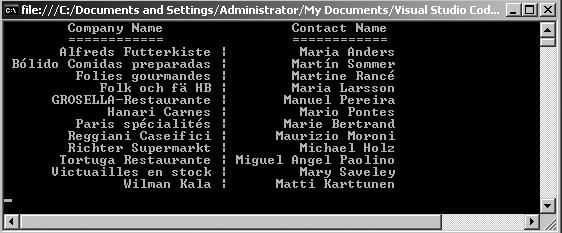
\includegraphics[width=\textwidth]{ado-rdr}
\end{center}
\end{frame}

\begin{frame}[fragile]
\frametitle{多结果集}
\begin{itemize}
\item NextResult() 方法可以用来访问多个结果集
\end{itemize}
\begin{lstlisting}
string sql1="SELECT companyname, contactname
            FROM customers WHERE companyname like 'A%';";
string sql2="SELECT firstname, lastname FROM employees;";

string sql = sql1 + sql2;
SqlCommand cmd = new SqlCommand(sql, conn);
SqlDataReader rdr = cmd.ExecuteReader();

do {
  while (rdr.Read())
  { Console.WriteLine("{0} : {1}", rdr[0], rdr[1]); }

  Console.WriteLine("Next Result Set");

}while(rdr.NextResult());
\end{lstlisting}
\end{frame}

\section{Data Set}

\begin{frame}
\frametitle{数据集 (\textit{DataSet})}
\begin{block}{\textit{DataSet}}
\CJKindent ADO.NET 的主要部件,作为从数据库中取出的数据在内存的缓存。由多个
 DataTable 组成,并可通过  DataRelation 相互关联;并且可用 UniqueConstraint
或 ForeignKeyConstraint 加强数据完整性。
\end{block}
\begin{center}
  %% Slides for ".NET Programming" by Chunyu Wang <chunyu@hit.edu.cn> %%

\begin{tikzpicture}[rounded corners, font=\sffamily\scriptsize, >=stealth]
\draw[fill=blue!20,fill opacity=.5] (0,0) rectangle (6,3.5); \draw (3,.2) node {DataSet};

\fill[white,sharp corners,shift={(.5,1)}] (0,0) rectangle + (1.5,1.2);
\draw[xstep=.3cm,ystep=.2cm, sharp corners,shift={(.5,1)}]
(0,0) grid +(1.5,1.2) (.75,-.2) node {DataTable};

\fill[white,sharp corners,shift={(4,.7)}] (0,0) rectangle + (1.5,1.2);
\draw[xstep=.3cm,ystep=.2cm, sharp corners,shift={(4,.7)}]
(0,0) grid +(1.5,1.2) (.75,-.2) node {DataTable};

\draw (3.5,2.75) node[fill=red!20,draw,ellipse] (r) {DataRelation};

\draw[->] (r) -- (2,2.2);
\draw[->] (r) -- (4.75,1.9);
\end{tikzpicture}

\end{center}
\end{frame}

\begin{frame}
\frametitle{数据集的特点}
\begin{itemize}
\setlength{\itemsep}{6pt plus 1pt}
\item 数据集相当于内存中的简化的数据库
\begin{itemize}
\item 数据来自数据源,可以随意更改
\item 可以将数据的更改更新到数据源
\item 可被串行化,可用于保存或通过网络传输
\end{itemize}
\item 数据集的组成
\end{itemize}
\begin{center}
  %% Slides for ".NET Programming" by Chunyu Wang <chunyu@hit.edu.cn> %%

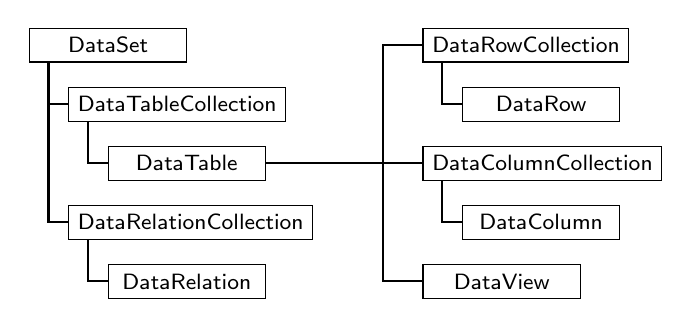
\begin{tikzpicture}
\tikzstyle{every node}=[anchor=west, draw, fill=white,
font=\sffamily\footnotesize, minimum width=2cm]
\foreach \x/\y/\t in 
  {0/4/DataSet, .5/3.25/DataTableCollection, 1/2.5/DataTable, .5/1.75/DataRelationCollection,
   1/1/DataRelation, 5/4/DataRowCollection, 5.5/3.25/DataRow, 5/2.5/DataColumnCollection,
   5.5/1.75/DataColumn, 5/1/DataView}
  \node at (\x,\y) (\t) {\t};
\draw[thick] (DataSet.south west) +(right:.25cm) |- (DataTableCollection);
\draw[thick] (DataTableCollection.south west) +(right:.25cm) |- (DataTable);
\draw[thick] (DataSet.south west) +(right:.25cm) |- (DataRelationCollection);
\draw[thick] (DataRelationCollection.south west) +(right:.25cm) |- (DataRelation);
\draw[thick] (DataTable.east) -- (4.5,2.5);
\draw[thick] (4.5,2.5) |- (DataRowCollection);
\draw[thick] (4.5,2.5) |- (DataColumnCollection);
\draw[thick] (4.5,2.5) |- (DataView);
\draw[thick] (DataRowCollection.south west) +(right:.25cm) |- (DataRow);
\draw[thick] (DataColumnCollection.south west) +(right:.25cm) |- (DataColumn);
\end{tikzpicture}

\end{center}
\end{frame}

\begin{frame}[fragile]
\frametitle{使用 DataSet 类}
\begin{center}
  
\begin{itemize}
\item 数据集  DynamicDS 中的 Customer 表
\end{itemize}
  \begin{tabular}{|l|l|l|l|}
    \hline
    \footnotesize \textbf{OrderID} & \footnotesize \textbf{FirstName} & \footnotesize \textbf{LastName} & \footnotesize \textbf{Date} \\
    \hline
    101              & John               & Doe               & 2006-9-1      \\
    \hline
    \dots            & \dots              & \dots             & \dots         \\
    \hline
  \end{tabular}
\end{center}
\begin{lstlisting}
DataSet ds = new DataSet("DynamicDS");
ds.Tables.Add("Customer");

ds.Tables["Customer"].Columns.Add("OrderID", 
                        Type.GetType("System.Int32"));
ds.Tables["Customer"].Columns.Add("FirstName", 
                        Type.GetType("System.String"));
ds.Tables["Customer"].Columns.Add("Date",
                        Type.GetType("System.DateTime"));

ds.Tables.Add("Order"); // another table
// ...
\end{lstlisting}
\end{frame}

\begin{frame}
\frametitle{DataSet 成员}
\begin{itemize}
\setlength{\itemsep}{8pt plus 1pt}
\item Clear 方法,清除所有数据表中的数据
\item Clone 方法,复制数据集的结构、模式等,数据除外
\item Copy 方法,复制结构和全部数据
\item Merge 方法,合并两个数据集
\item GetXml 方法,返回所有数据的 XML 表示形式
\item ReadXml 方法,从 XML 数据中读取数据
\item \texttt{\dots}
\end{itemize}
\end{frame}

\begin{frame}
\frametitle{DataTable 类}
\begin{itemize}
\setlength{\itemsep}{8pt plus 1pt}
\item DataTable 的列
\begin{itemize}
\setlength{\itemsep}{4pt plus 1pt}
\item 通过集合类型 DataColumnCollection 表示
\item 通过特性 Columns 访问
\item 描述表的定义,列的类型、约束等
\end{itemize}
\item DataTable 的行
\begin{itemize}
\setlength{\itemsep}{4pt plus 1pt}
\item 通过集合类型 DataRowCollection 表示
\item 通过特性 Rows 访问
\item 存储表的数据,一行一条记录
\end{itemize}
\end{itemize}
\end{frame}

\begin{frame}[fragile]
\frametitle{使用 DataTable 类示例}
\begin{lstlisting}
// ds is DataSet
DataTable myTable = ds.Tables["OrderDetail"];

foreach (DataColumn c in myTable.Columns)
{
   Console.Write(c.ColumnName + "\t");
}
Console.WriteLine("");

foreach (DataRow r in myTable.Rows){
  foreach (DataColumn c in myTable.Columns){
     Console.Write(r[c] + "\t");
  }
  Console.WriteLine("");
}

\end{lstlisting}
\end{frame}

\begin{frame}[fragile]
\frametitle{修改 DataTable 中的数据}
\begin{itemize}
\item 使用 DataRow 对象添加或修改记录
\item AcceptChanges, RejectChanges 等方法控制对数据的修改
\end{itemize}
\lstset{emph={AcceptChanges,RejectChanges}}
\begin{lstlisting}
DataTable tb = ds.Tables["Customer"];
DataRow  row = tb.NewRow();
row["OrderId"] = 102; row["FirstName"]="Mike"; ...

tb.Rows.Add(row);   tb.AcceptChanges();

DataRow r = tb.Rows[0];
r["FirstName"] = "Joe";
r.Delete();
tb.RejectChanges();
\end{lstlisting}
\end{frame}

\begin{frame}[fragile]
\frametitle{定义主键 (\textit{Primary Key})}
\begin{itemize}
\item 特性 PrimaryKey 可用于设置或获取表的主键
\item 设置主键只需赋值 DataColumn 数组
\end{itemize}
\lstset{emph={PrimaryKey}}
\begin{lstlisting}
workTable.PrimaryKey = new DataColumn[] 
                {workTable.Columns["CustLName"],
                workTable.Columns["CustFName"]};

// Or 

DataColumn[] myKey = new DataColumn[2]; 
myKey[0] = workTable.Columns["CustLName"]; 
myKey[1] = workTable.Columns["CustFName"];
workTable.PrimaryKey = myKey; 

\end{lstlisting}
\end{frame}

\begin{frame}[fragile]
\frametitle{约束 (\textit{Constraint})}
\begin{itemize}
\item UniqueConstraint
\end{itemize}
\lstset{emph={UniqueConstraint}}
\begin{lstlisting}
DataColumn[] myColumns = new DataColumn[2];
myColumns[0] = myTable.Columns["id"];
myColumns[1] = myTable.Columns["Name"];
UniqueConstraint myUC = 
  new UniqueConstraint("idNameCstrnt", myColumns, false);
myTable.Constraints.Add(myUniqueConstraint);
\end{lstlisting}
\begin{itemize}
\item ForeignKeyConstraint
\end{itemize}
\lstset{emph={ForeignKeyConstraint}}
\begin{lstlisting}
ForeignKeyConstraint custOrderFK = 
  new ForeignKeyConstraint ("Order_OrderDetail", 
      m_ds.Tables["Order"].Columns["OrderID"],       
      m_ds.Tables["OrderDetail"].Columns["fk_OrderID"]));

custOrderFK.DeleteRule = Rule.None;

custDS.Tables["OrderDetail"].Constraints.Add(custOrderFK); 
\end{lstlisting}
\end{frame}

\begin{frame}[fragile]
\frametitle{从数据库中导入数据}
\begin{itemize}
\item 首先创建 DataAdapter 和 DataSet
\item 通过 DataAdapter 的 Fill 方法填充 DataTable
\item 多次 Fill 可以添加并填充多个数据表
\end{itemize}
\lstset{emph={DataSet, Fill, SqlDataAdapter}}
\begin{lstlisting}[escapeinside=<>]
SqlCommand cmd = conn.CreateCommand();
cmd.CommandText = "SELECT Name, Age FROM Employees";

SqlDataAdapter da = new SqlDataAdapter();
da.SelectCommand = cmd;

DataSet ds = new DataSet();

da.Fill(ds, "NamesAndAges"); // <会自动执行 cmd>
\end{lstlisting}
\end{frame}

\begin{frame}[fragile]
\frametitle{填充并使用数据集}   %\attachfile[description=Populate DataSet]{code/PopDataSet.cs}
\begin{lstlisting}[escapeinside='']
string sql = "select productname,unitprice
         from products where unitprice < 20";

SqlConnection conn = new SqlConnection(connString);
SqlDataAdapter da = new SqlDataAdapter(sql, conn);
...
DataSet ds = new DataSet();
da.Fill(ds, "products"); //'表名products'
\end{lstlisting}
\pause
\begin{lstlisting}[escapeinside='']
DataTable dt = ds.Tables["products"]; //'访问表'

foreach (DataRow row in dt.Rows){     //'访问行'

  foreach (DataColumn col in dt.Columns)
    Console.WriteLine(row[col]);      //'访问数据'

  Console.WriteLine("".PadLeft(20, '='));
}
\end{lstlisting}
\end{frame}

\begin{frame}
\frametitle{更新数据库}
\begin{itemize}
\item DataAdapter 加载数据后,所有更新都发生在数据集中
\item 要更新数据源,需要使用  DataAdapter 的相应方法
  \begin{itemize}
  \item Update 方法检查相应的数据集
  \item InsertCommand, DeleteCommand, UpdateCommand 更新DBMS
  \end{itemize}
\end{itemize}
\begin{center}
  %% Slides for ".NET Programming" by Chunyu Wang <chunyu@hit.edu.cn> %% -*- coding: utf-8 -*-

\begin{tikzpicture}[rounded corners, font=\scriptsize, >=stealth]
\draw[fill=yellow!30, fill opacity=.5] (-1,.8) rectangle (6,6);
\draw[fill=blue!20, fill opacity=.8] (-.8,1) rectangle (2,4.5);
\draw[fill=blue!20, fill opacity=.8] (2.2,1) rectangle (5.8,5.8);
\draw (.6,4.1) node {\bf Client} 
      (4,5.4) node {\bf .NET Framework}
      (4,5.1) node {\bf Data Provoder};
\draw (3.3,4.5) node[inner xsep=0pt,fill=red!20,draw,ellipse]  (da) {DataAdapter};
\draw (4.5,3.5) node[inner xsep=0pt,fill=red!20,draw,ellipse]  (ic) {InsertCommand};
\draw (4.1,2.5) node[inner xsep=0pt,fill=red!20,draw,ellipse]  (uc) {UpdateCommand};
\draw (3.5,1.5) node[inner xsep=0pt,fill=red!20,draw,ellipse]  (dc) {DeleteCommand};

\draw[fill=blue!20] (7.5,2.3) ellipse (.5cm and .15cm);
\fill[sharp corners,blue!20] (7,2.3) rectangle (8,3);
\draw[fill=blue!20] (7.5,3) ellipse (.5cm and .15cm);
\draw (7,2.3) -- (7,3) (8,2.3) -- (8,3);
\draw (7.5,2.6) node {DBMS};

\draw (.6,2.45) circle (1.15cm);
\fill[white,sharp corners,shift={(-.15,1.95)}] (0,0) rectangle + (1.5,1);
\draw[xstep=.3cm,ystep=.2cm, sharp corners,shift={(-.15,1.95)}] (0,0) grid +(1.5,1);

\draw (.5,3.2) node {DataSet} (.5,1.7) node {DataTable};

\draw[->] (.6,2.45) ++(60:1.15cm) -- (da.190);
\draw[->,dashed] (da.270) -- (ic.170);
\draw[->,dashed] (da.240) -- (uc.165);
\draw[->,dashed] (da.220) -- (dc.170);

\draw[->] (ic.east) .. controls +(right:1cm) and +(120:.1cm) ..  (7,3);
\draw[->] (uc.east) .. controls +(right:1cm) and +(left:.1cm) ..  (7,2.5);
\draw[->] (dc.east) .. controls +(right:1cm) and +(210:.1cm) ..  (7,2.3);
\end{tikzpicture}

\end{center}
\end{frame}

\begin{frame}[fragile]
\frametitle{更新数据库示例}
\lstset{emph={Update,UpdateCommand}}
\begin{lstlisting}
SqlDataAdapter dataAdpater = new SqlDataAdapter(
   "SELECT ID, Name FROM Categories", connection);

dataAdpater.UpdateCommand = new SqlCommand(
   "UPDATE Categories SET Name = @Name " +
   "WHERE ID = @ID" , connection);
// then parameters setup

DataSet dataSet = new DataSet();
dataAdpater.Fill(dataSet, "Categories");   

DataRow row = dataSet.Tables["Categories"].Rows[0];
row ["Name"] = "New Category";

dataAdpater.Update(dataSet, "Categories");
\end{lstlisting}
参考 \href{http://msdn2.microsoft.com/zh-cn/library/33y2221y.aspx}
{\beamergotobutton{\scriptsize 代码完整版}}
\end{frame}

\begin{frame}[fragile]
\frametitle{增加数据示例} %\attachfile[description=Update DataBase]{code/PersistAdd.cs}
\begin{lstlisting}
string qry="select firstname,lastname from employees";

SqlDataAdapter da = new SqlDataAdapter();
da.SelectCommand = new SqlCommand(qry, conn);
DataSet ds = new DataSet();
da.Fill(ds, "employees");

DataTable dt = ds.Tables["employees"];
DataRow newRow = dt.NewRow();
newRow["firstname"] = "Roy";
newRow["lastname"] = "Beatty";
dt.Rows.Add(newRow);
...
\end{lstlisting}
\end{frame}

\begin{frame}[fragile]
\frametitle{增加数据示例(续)}
\begin{lstlisting}[escapeinside='']
...
string ins="insert into employees( firstname, lastname)
                           values(@firstname,@lastname)";

SqlCommand cmd = new SqlCommand(ins, conn);

//'设置参数类型'
cmd.Parameters.Add("@firstname",
                 SqlDbType.NVarChar, 10, "firstname");
cmd.Parameters.Add("@lastname",
                 SqlDbType.NVarChar, 20,  "lastname");

da.InsertCommand = cmd;
da.Update(ds, "employees");
\end{lstlisting}
\end{frame}

\begin{frame}
\frametitle{连接模型和无连接模型}
\begin{itemize}
  \setlength{\itemsep}{8pt plus 1pt}
\item 连接模型
  \begin{itemize}
    \setlength{\itemsep}{6pt plus 1pt}
  \item 使用 DataReader 访问数据库,需要始终保持数据库的连接
  \item 内存的使用较少,适合大数据量的处理
  \end{itemize}
\item 无连接模型
  \begin{itemize}
    \setlength{\itemsep}{6pt plus 1pt}
  \item 使用 DataAdapter 填充数据表后,自动断开连接
  \item 需要的时候会自动连接,比如更新数据源
  \item 方便随时更新数据库
  \end{itemize}
\end{itemize}
\end{frame}

\begin{frame}
\frametitle{ADO.NET 和 XML}
\begin{itemize}
\item ADO.NET 和 XML 紧密集成
\item DataSet 提供了多种 XML 数据的处理方法
\item DataSet 可以作为 XML 和关系数据的转换中介
\end{itemize}
\begin{center}
  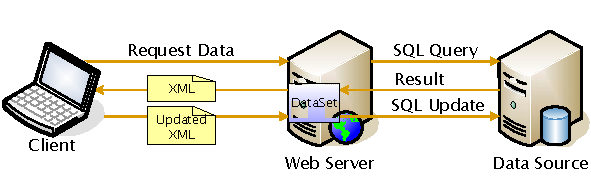
\includegraphics[width=\textwidth]{ado-xml}
\end{center}
\end{frame}

\begin{frame}[fragile]
\frametitle{使用 XML 保存数据和模式}
\begin{itemize}
\item 分别保存 XML 数据和模式
\end{itemize}
\lstset{emph={WriteXmlSchema,WriteXml}}
\begin{lstlisting}
DataSet ds = new DataSet("films");
DataTable da = ds.Table.Add("Movies");
...
da.Fill(dt);

ds.WriteXmlSchema("C:\\movies_schema.xsd");
ds.WriteXml("C:\\movies_data.xml");

\end{lstlisting}
\begin{itemize}
\item 将模式和数据保存在一个 XML 文件中
\end{itemize}
\begin{lstlisting}

ds.WriteXml("all.xml",XmlWriteMode.WriteSchema);

\end{lstlisting}
\end{frame}

\begin{frame}[fragile]
\frametitle{从 XML 恢复 DataSet}
\begin{itemize}
\item 使用已有的 XML 模式构造 DataSet
\end{itemize}
\begin{lstlisting}
DataSet ds = new DataSet();
ds.ReadXmlSchema ("d:\\movie_schema.xsd");

DataTable tb = ds.Table[0];
\end{lstlisting}
\begin{itemize}
\item 从 XML 读入数据
\end{itemize}
\begin{lstlisting}
DataSet ds = new DataSet();
ds.ReadXml("C:\\movie_data.xml");

\end{lstlisting}
\end{frame}

\section{数据绑定}

\begin{frame}
\frametitle{窗体控件的数据绑定}
\begin{block}{数据绑定}
  \CJKindent 数据绑定是一种将控件内容与底层数据源链接的方式,对中间数据源的改动
  会自动反映到与之绑定的数据控件上,而对数据控件的修改也能自动回送给中间数据源。
\end{block}
\begin{itemize}
\setlength{\itemsep}{8pt plus 1pt}
\item 中间数据源不是外部的数据库
\item 控件不能通过活动的连接直接与数据源绑定
\item 绑定只限于数据的内存表示,如数据集等
\end{itemize}
\end{frame}

\begin{frame}[fragile]
\frametitle{简单数据绑定}
\begin{itemize}
\item 通过集合 DataBindings,所有控件都能使用单值数据绑定
\item 将数据源于控件的一个或多个属性链接
\end{itemize}
\begin{lstlisting}
txtUnitCost.DataBindings.Add("Text", dt, "UnitCost");
\end{lstlisting}
\begin{itemize}
\item 将 DataTable dt 中 UnitCost 列的第一个值显示在文本框中
\item 参数的含义:
\begin{itemize}
  \item \verb|"Text"| --- 特性的名字,.NET 使用反射找到相应特性
  \item \verb|dt| --- 数据源,如 DataTable
  \item \verb|"UnitCost"| --- 数据源中的字段名
  \end{itemize}
\end{itemize}
\end{frame}

\begin{frame}[fragile]
\frametitle{简单数据绑定示例}
\begin{lstlisting}
private void
MultipleControlBinding_Load(object sender, EventArgs e)
{
  // Get the data object.
  DataTable dt = Program.StoreDB.GetProducts();

  // Use complex binding.
  cboModelName.DataSource = dt;
  cboModelName.DisplayMember = "ModelName";

  // Use simple binding.
  lblModelNumber.DataBindings.Add(
                              "Text", dt, "ModelNumber");
  lblUnitCost.DataBindings.Add(
                              "Text", dt, "UnitCost");
  lblDescription.DataBindings.Add(
                              "Text", dt, "Description");
}
\end{lstlisting}
\end{frame}

\begin{frame}[fragile]
\frametitle{与列表控件的复杂绑定}
\begin{itemize}
\item 当控件包含数据源及其成员或特性时,使用复杂绑定
\begin{itemize}
\item 如 ListBox, CheckedListBox, DataGrid, DataGridView 等
\end{itemize}
\item 复杂绑定允许控件绑定到数据集上,同时显示多个数据
\item 控件至少需要设置 DataSource 和 DisplayMember 两个属性
\end{itemize}
\lstset{emph={DataSource, DisplayMember}}
\begin{lstlisting}
da.Fill(ds, "movies");
DataTable dt = ds.Tables[0];

listBox1.DataSource = ds;
listBox1.DisplayMember = "movies.Title";

// optional property
listBox1.ValueMember = "movies.ID";
\end{lstlisting}
\end{frame}

\begin{frame}[fragile]
\frametitle{绑定管理器}
\begin{itemize}
\item 数据源都有一个绑定管理器,负责跟踪数据源的所有连接
\item 如果数据源更新,管理器负责更新相应控件
\item 如果控件有更改,负责改变数据源中的数据
\item 管理器的成员
\begin{itemize}
\item Binding 类,维护控件特性和某对象特性之间的简单绑定
\item CurrencyManager 类,管理 Binding 对象的列表
\item PropertyManager 类\\维护对象的特性与数据绑定控件特性之间的 Binding
\item BindingContext 类\\链接到特定控件的 BindingManagerBase 集合上
\end{itemize}
\end{itemize}
\end{frame}

\begin{frame}[fragile]
\frametitle{BindingManagerBase 浏览列表}
\begin{itemize}
\item 在数据源列表元素间移动,同时更新列表绑定的控件内容
\end{itemize}
\begin{lstlisting}
listBox1.DataSource = ds;
listBox1.DisplayMember = "movies.Title";

txtStudio.DataBinding.Add("text",ds,"movies.studio");

BindingManagerBase bmb;
bmb = this.BindingContext[ds,"movies"];
bmb.PositionChanged += bmb_PositionChanged;

private bmb_PositionChanged(object s, EventArgs e){
  bmb.Position++;
}
\end{lstlisting}
\end{frame}

\begin{frame}
\frametitle{Visual Studio 中的配置数据源}
\begin{itemize}
\item 菜单中选 Data/Add New Data Source 配置数据源
\end{itemize}
\begin{figure}
  \centering
  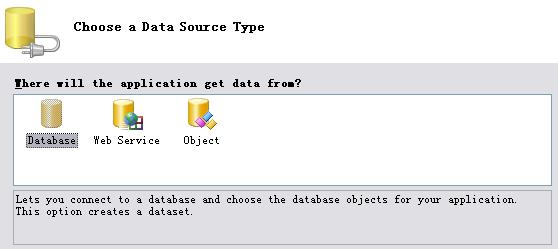
\includegraphics[width=\textwidth]{ado-source01}
\end{figure}

\end{frame}

\begin{frame}
\frametitle{Visual Studio 中的配置数据源}
\begin{itemize}
\item 根据提示设置 Connection String
\end{itemize}
\begin{figure}
  \centering
  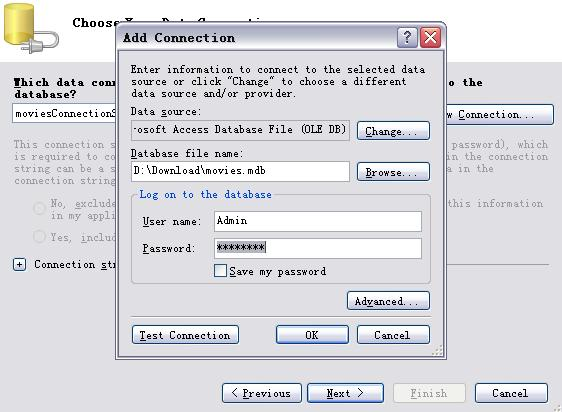
\includegraphics[width=\textwidth]{ado-source02}
\end{figure}
\end{frame}

\begin{frame}
\frametitle{向项目添加数据集}
\begin{itemize}
\item 菜单中选 Project/Add New Item 可以添加各种控件或组件
\end{itemize}
\begin{figure}
  \centering
  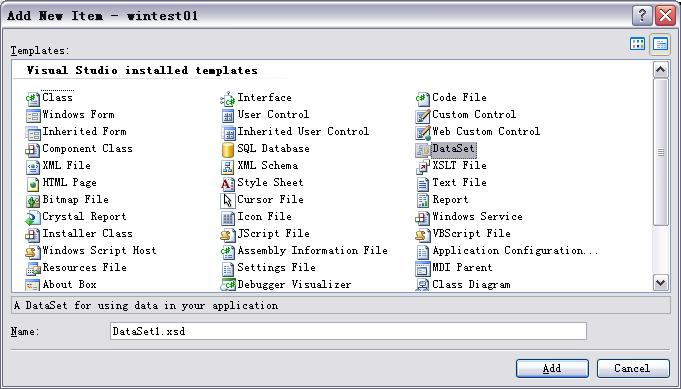
\includegraphics[width=\textwidth]{ado-dataset01}
\end{figure}
\end{frame}

\begin{frame}
\frametitle{使用可视化工具设计数据集}
\begin{itemize}
\item 在 Data Source 窗口中浏览数据集
\item 右键选择 Designer 中编辑
\end{itemize}
\begin{figure}
  \centering
  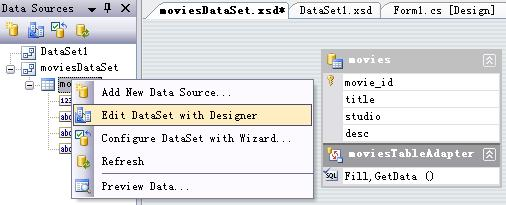
\includegraphics[width=.8\textwidth]{ado-dataset02}
\end{figure}
\end{frame}

\begin{frame}
\frametitle{通过拖拽绑定控件}
\begin{itemize}
\item 拖拽 DataSet 到窗体,可以自动生成一些控件和组件
\end{itemize}
\begin{figure}
  \centering
  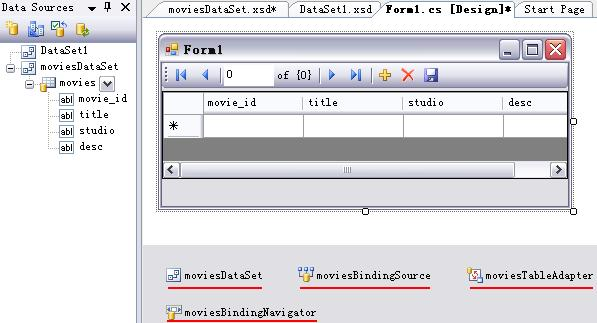
\includegraphics[width=\textwidth]{ado-binding01}
\end{figure}
\end{frame}

\begin{frame}
\frametitle{通过拖拽绑定控件}
\begin{itemize}
\item 修改 DataColumn 显示为各种控件
\item 拖拽 DataColumn 到窗体,自动生成绑定的控件
\end{itemize}
\begin{figure}
  \centering
  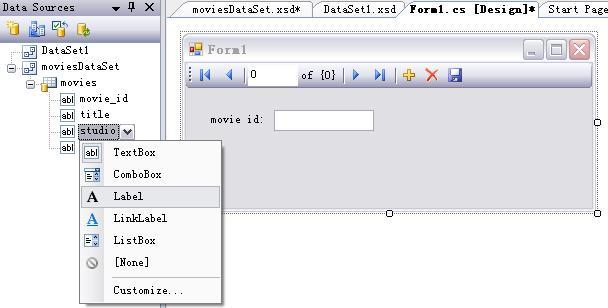
\includegraphics[width=\textwidth]{ado-binding02}
\end{figure}
\end{frame}


% Local Variables:
% mode: LaTeX
% TeX-master: "part-06.tex"
% TeX-header-end: "% End-of-Header$"
% TeX-trailer-start: "% Start-of-Trailer$"
% coding: utf-8
% End:

